\chapter{Preliminary Evaluation}
To evaluate the above mentioned research questions, a preliminary evaluation is conducted. Optimizing and improving our approach with the help of feedback from the participants is the primary goal of this master thesis. Further, we want to learn which status and moods knowledge workers share with their closest team members, what they learn from their team-mates' sharing and the overall impact on their perception of workplace isolation. The three main areas of interest and the research questions we would like to answer with the study are as follows:

TODO: Add research questions

TODO: Quickly describe \autoref{fig:study_timeline} in words before jumping into more details in the following sections.

\begin{figure}[h]
    \centering
    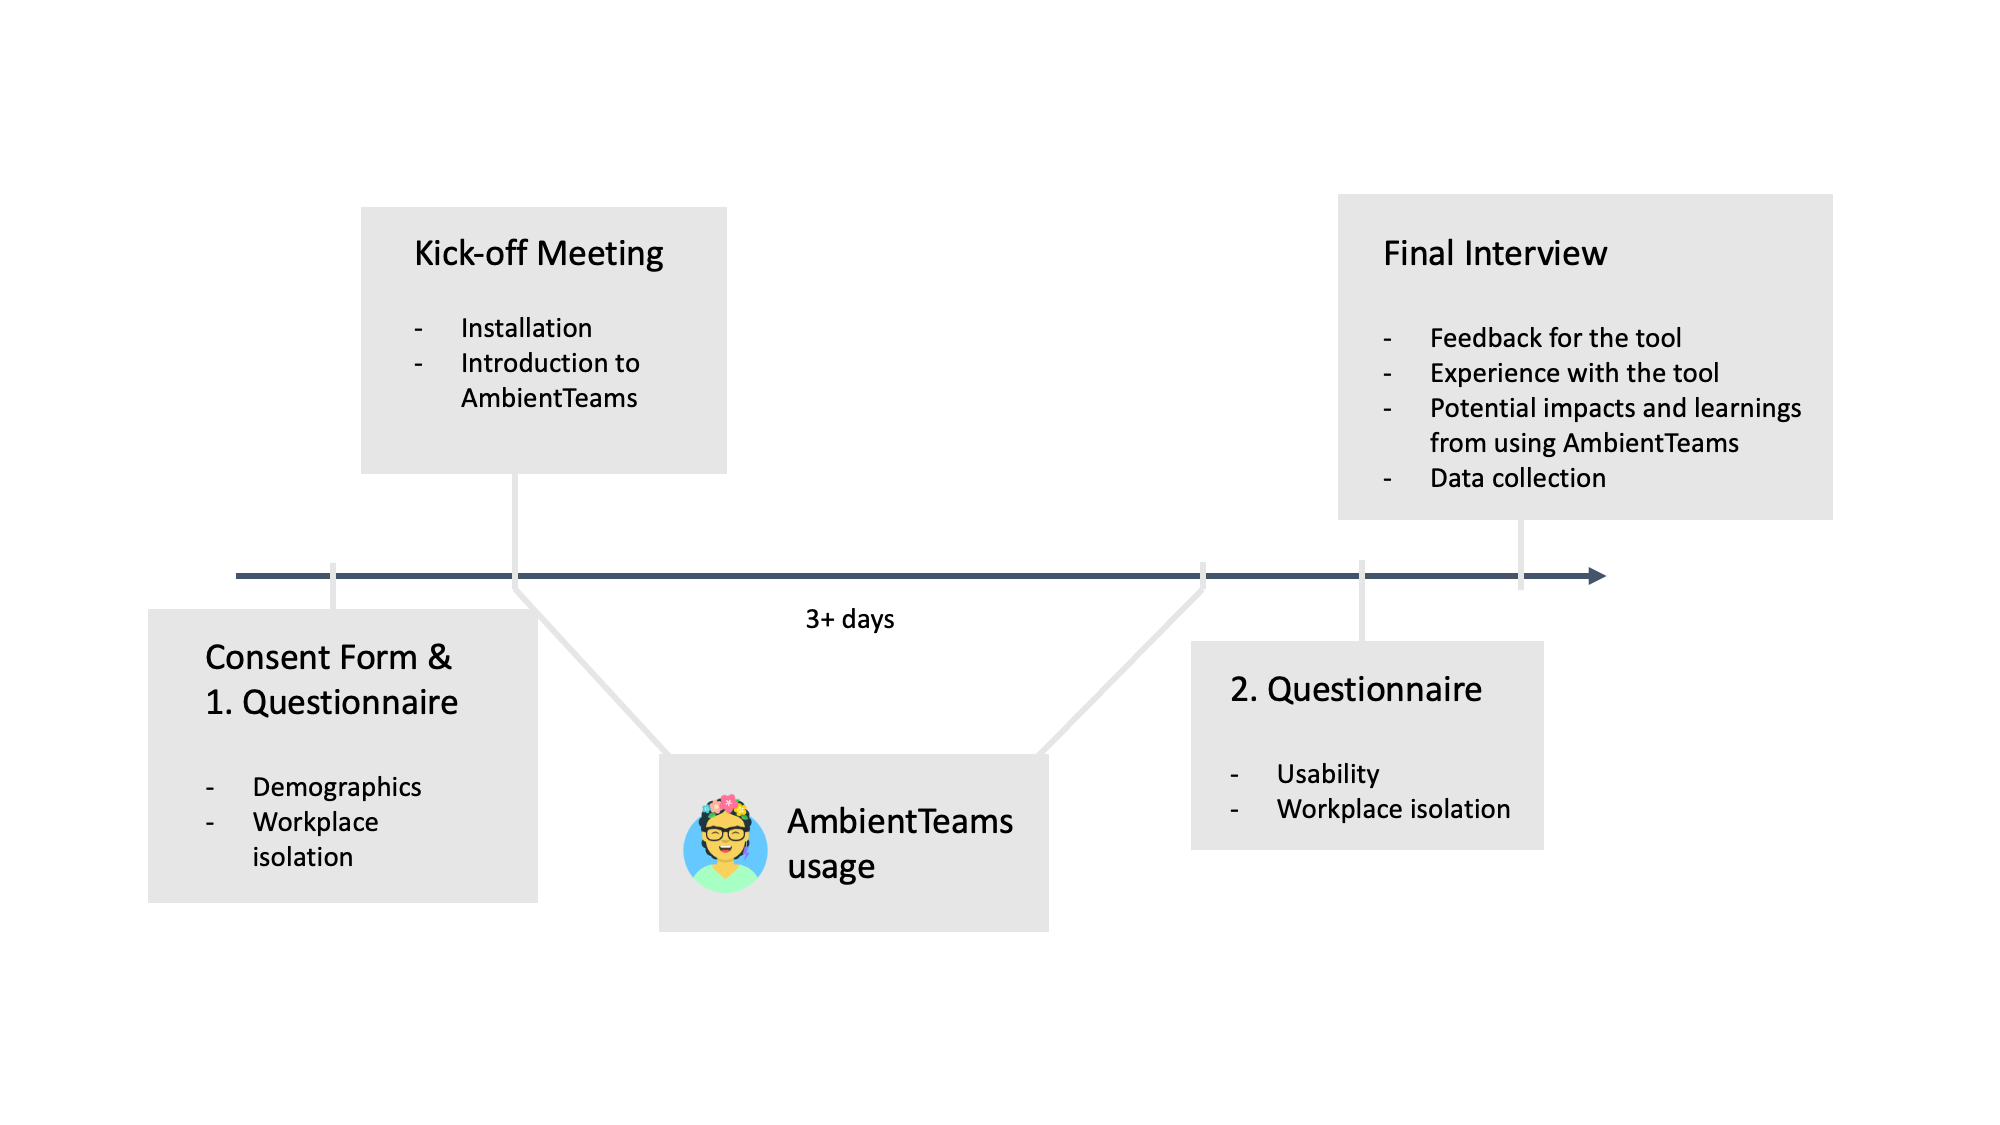
\includegraphics[width=.8\linewidth]{./images/Study_Timeline.png}
    \caption{Study timeline}
    \label{fig:study_timeline}
\end{figure}

\section{Participants Recruitment}
\label{section:recruitment}
As a first step, an interested team had to be recruited. To that end, the researchers' personal network will be used. To that purpose, the study description is forwarded to the contacts, and once an interested team has been identified, it is checked whether it fulfills the participation criteria and if the prospective participants are (technically) allowed to install AmbientTeams on their computer. If this is not the case, the company's consent and approval to install AmbientTeams is first obtained. To provide the company with as much information as possible about the study and the privacy/confidentiality of the data collected during the study, the consent form and a study description will be given to the company for review. After gaining the company's approval, the individual interested team members are approached by presenting the study, discussing the steps and goals of the study, and emphasizing that participation is entirely voluntary.

The requirements for teams participating were as follows:

\begin{enumerate}
    \item At least three team members
    \item Three or more common working days a week
    \item Spending the majority of their workday on the computer
    \item Having all the required rights to install AmbientTeams on their work computer
    \item Willingness to use AmbientTeams during at least three full days of work (approximately 0800 - 1700)
    \item Using macOS or Microsoft Windows
    \item An active internet connection
\end{enumerate}

\section{Participants}
With our recruitment, we were able to find an interested team. TODO: Describe team

\section{Initial meeting}
\label{section:initial_meeting}
Installation

\section{Prestudy Questionnaire}
\label{section:prestudy_questionnaire}
The questions are taken from ....

\section{Evaluation Phase}
\label{section:evaluation}
How long? \\
During the study notes from notion

\section{Poststudy Questionnaire}
\label{section:poststudy_questionnaire}
The questions are taken from ....

\section{Interview}
\label{section:interview}
Interview questions and their relevance for the research questions